\documentclass[11pt,a4paper]{article}

% Basic packages
\usepackage[a4paper,margin=1.8cm]{geometry}
\usepackage{graphicx}
\usepackage{hyperref}
\usepackage{enumitem}

% Simple settings
\pagenumbering{gobble}
\setlength{\parindent}{0pt}
\setlist[itemize] {itemsep=2pt, topsep=3pt}

\begin{document}

% -------------------- HEADER --------------------

\begin{center}
    % Add your photo by keeping profile.png in the same folder
    % 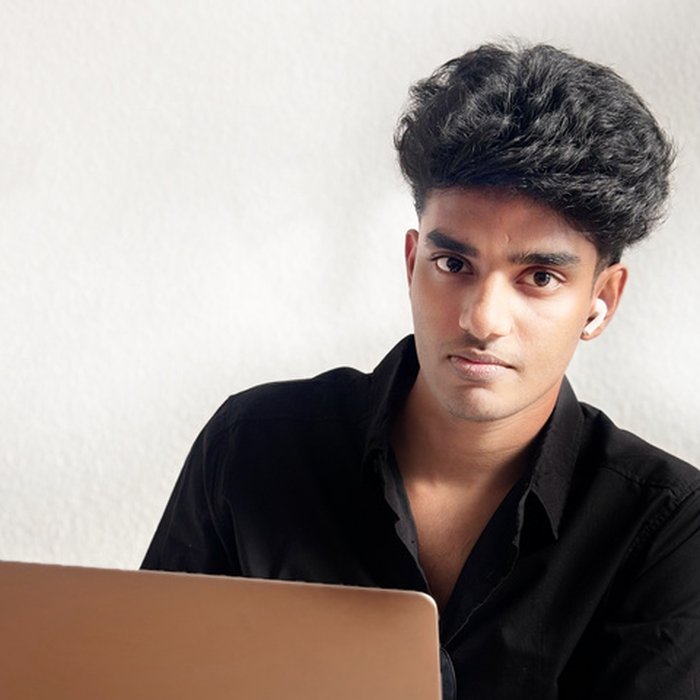
\includegraphics[width=3cm]{profile.png}

    \vspace{0.2cm}

    {\LARGE \textbf{Arjun Bijoy}}\\
    \vspace{0.1cm}
    Software Engineering Student\\
    \vspace{0.2cm}

    Berlin, Germany \\
    Phone: +49 176 24734571 \\
    Email: \href{mailto:arjunbijoy1917r@gmail.com}{arjunbijoy1917r@gmail.com} \\
    LinkedIn: \href{https://linkedin.com/in/arjun-bijoy-0b93b8380}{linkedin.com/in/arjun-bijoy-0b93b8380} \\
    GitHub: \href{https://github.com/arjunbijoy1917r-cmyk}{github.com/arjunbijoy1917r-cmyk} \\
    Portfolio: To be added
\end{center}

\vspace{0.3cm}
\hrule
\vspace{0.4cm}

% -------------------- PROFILE --------------------

\section*{Profile}

I am a Software Engineering student at GISMA University of Applied Sciences in Berlin. I am currently learning Python, Java, HTML, CSS, SQL, and basic LaTeX through university work and personal practice projects.

I am interested in software development, databases, and practical problem solving.  by step and using my projects to show my learning progress.

% -------------------- EDUCATION --------------------

\section*{Education}

\textbf{Bachelor of Software Engineering} \\
GISMA University of Applied Sciences, Berlin, Germany \\

\vspace{0.2cm}

\textbf{Higher Secondary Education} \\
Bio-Maths, India \\
Completed in 2024

% -------------------- SKILLS --------------------

\section*{Skills}

\begin{itemize}
    \item Basic Python programming
    \item Basic Java programming
    \item HTML and CSS
    \item SQL databases
    \item Basic LaTeX documentation
    \item Problem solving
    \item Teamwork and communication
\end{itemize}

% -------------------- PROJECTS --------------------

\section*{Projects}

\textbf{Python University System} \\

A simple Python project for managing university-related data such as students, courses, instructors, and enrollments. I used basic classes and objects to organize the program.

GitHub: \href{https://github.com/arjunbijoy1917r-cmyk/python-university-system}{github.com/arjunbijoy1917r-cmyk/python-university-system}

\vspace{0.3cm}

\textbf{University Database Project} \\

A university management database project created using SQL. It includes tables for students, courses, instructors, and enrollments, along with sample data and basic queries.

GitHub: \href{https://github.com/arjunbijoy1917r-cmyk/university_database_project}{github.com/arjunbijoy1917r-cmyk/university_database_project}

% -------------------- EXPERIENCE --------------------

\section*{Experience}

\textbf{Restaurant Work Experience}

\begin{itemize}
    \item Took customer orders and helped with daily restaurant service.
    \item Kept the dining area clean and organized during shifts.
    \item Handled cash and card payments.
    \item Worked with colleagues in English and basic German.
\end{itemize}

\vspace{0.2cm}

\textbf{Academic and Technical Exercises}

\begin{itemize}
    \item Practiced Python, HTML, CSS, SQL, and LaTeX as part of university work.
    \item Created simple web pages and database project files.
    \item Learned how to organize project folders, write basic documentation, and upload work to GitHub.
\end{itemize}

% -------------------- LANGUAGES --------------------

\section*{Languages}

\begin{itemize}
    \item Malayalam - Mother tongue
    \item English - Good communication
    \item German - Basic to intermediate, still improving
\end{itemize}

% -------------------- ADDITIONAL INFORMATION --------------------

\section*{Additional Information}

\textbf{Nationality:} Indian \\  
\textbf{Date of Birth:} 02 August 2006

\end{document}

